\section{Background and Related works}

 % $\Delta W_n^t$
 
Federated learning has demonstrated efficacy in an array of imaging modalities, including Magnetic Resonance Imaging (MRI) \cite{sheller2020federated}\cite{silva2019federated}, X-ray \cite{balachandar2020accounting}, retinal imaging \cite{balachandar2020accounting}, as well as in applications such as brain tumor segmentation \cite{bakas2017advancing}\cite{lee2018privacy}, diagnosis \cite{pan2019improving}, and treatment selection \cite{lee2018privacy}. In particular, Federated Learning (FL) has proven to be a valuable tool for supporting physicians in their decision-making process regarding the treatment of COVID-19 patients. A landmark study that involved 20 institutions across five continents found that FL played a significant role in shaping patient treatment plans\cite{flores2021federated}. The study employed chest radiography images in conjunction with clinical information to determine the appropriate level of care and oxygen requirements for patients afflicted with COVID-19. It was observed that FL improved the performance of the predictive model, especially for institutions with smaller datasets, compared to using only local data for model training. Additionally, it was found that healthcare facilities with smaller datasets often had underrepresented categories due to a low number of patients in certain classes. The implementation of FL led to a notable improvement in predictions for these underrepresented patient categories.

\begin{figure*}[t!]
\centering
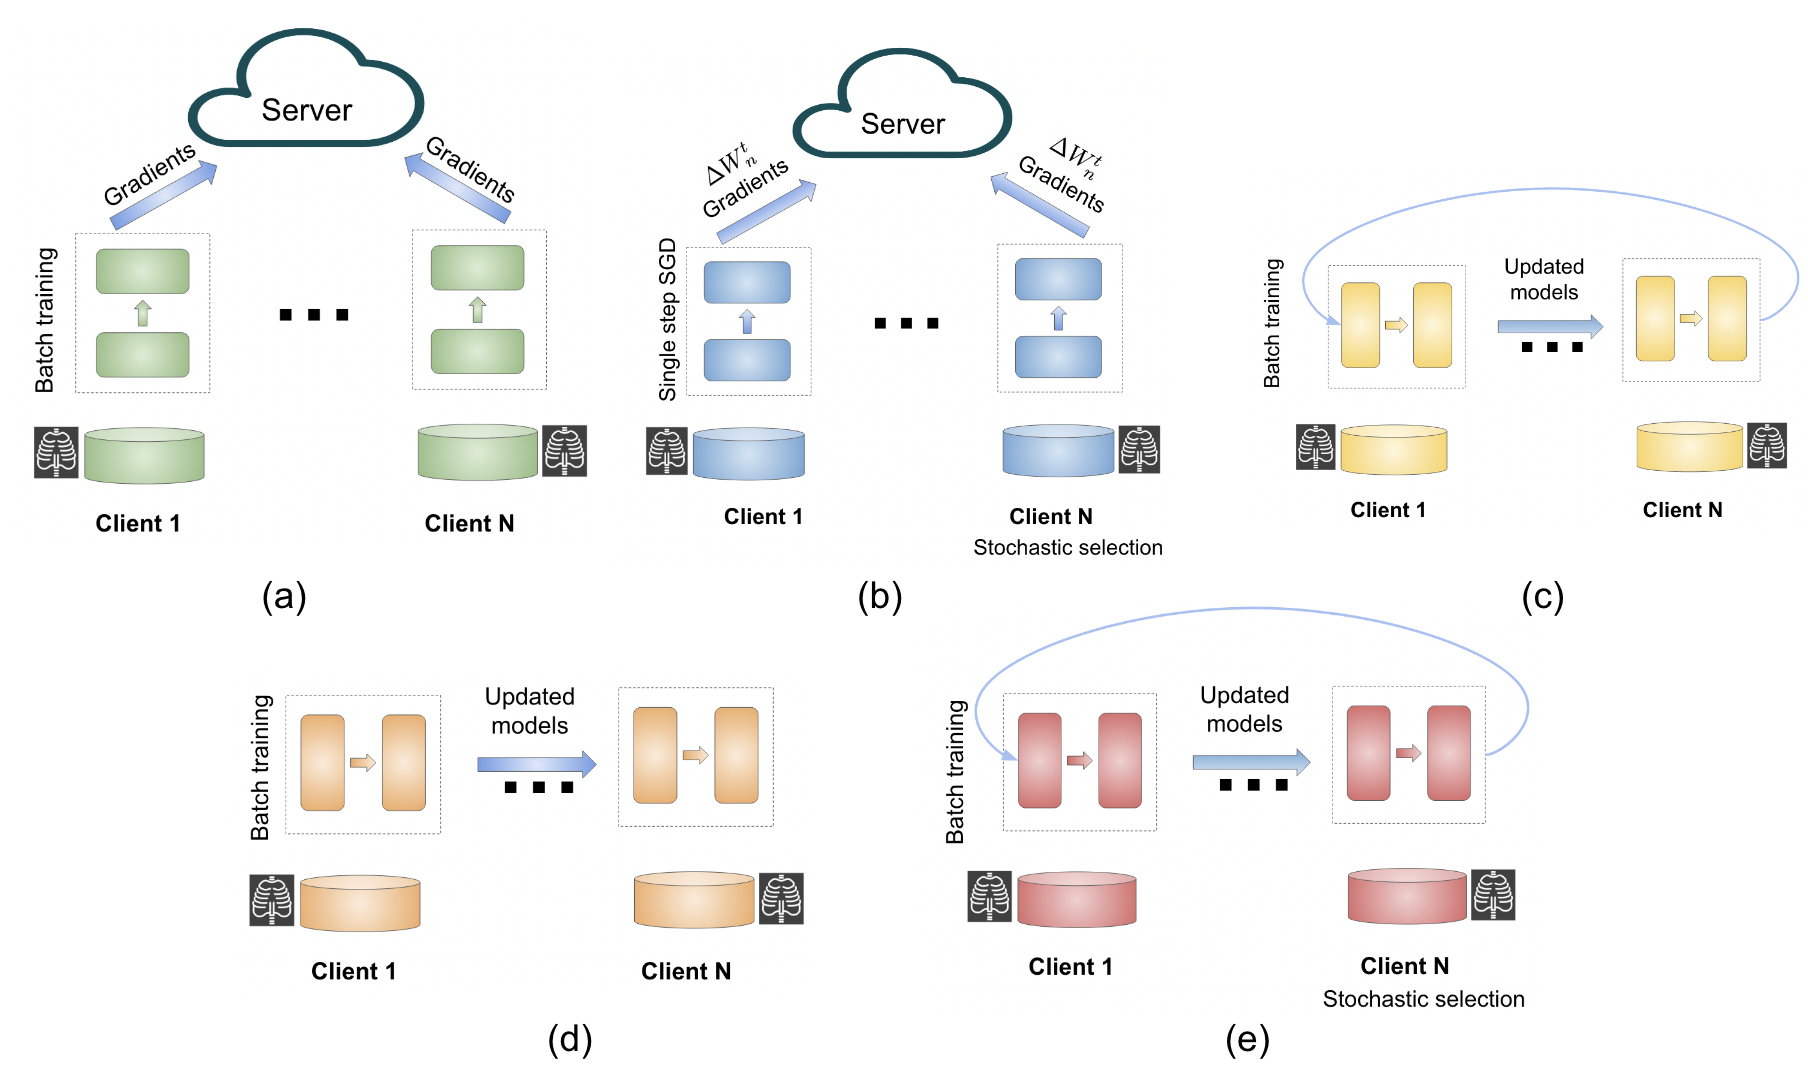
\includegraphics[width=1\textwidth]{FLmodels.png}
\caption{Illustration of FL models and algorithms: (a) Federated averaging, where clients train on a local batch of data. (b) FedSGD, in which a subset of clients is selected, and each performs a single step of SGD before sending model updates to the server. (c) Cyclic Weight Transfer (CWT), where clients train locally and pass the model to the next client, repeating the cycle. (d) Single Weight Transfer (SWT), where the model passes through each client only once. (e) Stochastic Weight Transfer (STWT), in which the model is sequentially passed through clients, with participating clients in each round being sampled randomly.}
\label{fig:flalgorithms}
\end{figure*}


Recent research has focused on the classification of scan images to distinguish between COVID-19 patients and healthy individuals, as well as identifying lesion areas. The primary application of AI in managing COVID-19 patients has been the interpretation of radiology images, especially chest CT scans.  The detection of lung alterations through these scans plays an important role in optimizing patient management and guiding treatment decisions\cite{yan2020interpretable}\cite{hu2020challenges}\cite{burian2020intensive}.  Several studies have also explored 3D Convolutional neural networks \cite{wang2020weakly} and COVID-19 detection with a limited number of training samples.

While the majority of these studies report favorable accuracy, they often presume a centralized environment wherein a single data center has access to all data. However, a few studies have successfully applied distributed learning for COVID-19 detection, employing global aggregation models such as model averaging in federated learning settings\cite{ho2022fedsgdcovid}\cite{zhang2021dynamic}, or within a blockchain framework \cite{kumar2021blockchain}. These studies have pointed to certain limitations of existing algorithms, such as high communication overhead \cite{remedios2020federated}, as well as convergence issues or catastrophic forgetting when the number of participating hospitals increases \cite{sheller2020federated} \cite{chang2018distributed}.


To our knowledge, no study has been performed that compared multiple FL algorithms under standard conditions to evaluate their applicability. Therefore, comparing multiple FL algorithms under standard conditions could be informative in evaluating their applicability in practice.

To evaluate the existing methods from multiple perspectives, we have implemented the most popular models and compared them in terms of performance, communication overhead, and computation burden.